\documentclass[12pt]{article}
\usepackage[myheadings]{fullpage}
\usepackage{fancyhdr}
\usepackage{lastpage}
\usepackage{graphicx}
\usepackage{caption}
\usepackage{subcaption}
\usepackage{amsfonts}
\usepackage{amsmath} 
\usepackage{amsthm}
\usepackage{amssymb}
\usepackage{tabu}
\usepackage{mathrsfs}
\usepackage{graphicx}
\usepackage{xtab}
\usepackage{algorithm}
\usepackage{algpseudocode}
\usepackage{wrapfig}
\usepackage{empheq}
\usepackage{pdfpages}

%-------------------------------------------------------------------------------
% NEW MATH COMMANDS
%-------------------------------------------------------------------------------
\newcommand{\N}{\mathbb{N}}
\newcommand{\R}{\mathbb{R}}
\newcommand{\Z}{\mathbb{Z}}
\newcommand{\K}{\mathbb{K}}
\newcommand{\Q}{\mathbb{Q}}
\newcommand{\Sp}{\mathbb{S}}
\newcommand{\pd}{\partial}
\newcommand{\cC}{\mathscr{C}}
\newcommand{\p}{\rho}
\newcommand{\y}{\gamma}
\newcommand{\re}{\, \mathfrak{R}}
\newcommand{\norm}[1][u]{\left\Vert #1 \right\Vert}
\newcommand{\e}{\, \varepsilon}
\newcommand{\lnorm}[1][u]{\norm[#1]_{L^2}}
\newcommand{\hnorm}[2][1]{\norm[#2]_{H^{#1}}}
\newcommand{\dl}{\, \delta}
\newcommand{\hf}{\, \frac{1}{2}}
\newcommand{\cdom}{\mathscr{D}_{1}^{\infty}}
\newcommand{\cadom}{\mathscr{D}_{0,1}^{\infty}}
\newcommand{\dom}{\, \mathcal{D}}
\newcommand{\Lds}[1][s]{\hat{L}_{#1}^{\dag}}
\newcommand{\w}{\omega}
\newcommand{\tw}{\tilde{\w}}
\newcommand{\vp}{\varphi}
\newcommand{\Lam}{\Lambda}
\newcommand{\M}{\mathcal{M}}
\DeclareMathOperator{\Ric}{Ric}
\DeclareMathOperator{\sympl}{Sympl}
\DeclareMathOperator{\tr}{tr}
\DeclareMathOperator{\xd}{d}
\DeclareMathOperator{\J}{J}
\DeclareMathOperator{\Rm}{Rm}
\DeclareMathOperator{\Vol}{Vol}
\DeclareMathOperator{\brg}{K}
\DeclareMathOperator{\hess}{Hess}
\DeclareMathOperator{\Supp}{Supp}
\DeclareMathOperator{\End}{End}
\DeclareMathOperator{\Lip}{Lip}
\DeclareMathOperator{\im}{Im}
\DeclareMathOperator{\rank}{rank}
\DeclareMathOperator{\Span}{Span}
\DeclareMathOperator{\Nil}{Nil}
\newcommand{\hu}{\hat{u}}
\newcommand{\C}{\mathbb{C}}
\newcommand{\A}{\mathbf{A}}
\newcommand{\mfld}{\mathcal{M}}
\newcommand{\zba}[1][\alpha]{\bar{z}^{#1}}
\newcommand{\zbb}[1][\beta]{\bar{z}^{#1}}
\newcommand{\za}[1][\alpha]{z^{#1}}
\newcommand{\zb}[1][\beta]{z^{#1}}
\newcommand{\al}{\alpha}
\newcommand{\be}{\beta}
\newcommand{\proj}{\mathbb{P}}
\newcommand{\lie}{\mathcal{L}}
\newcommand{\dd}{\pd \bar{\pd}}
\newcommand{\Om}{\Omega}
\newcommand{\pdb}{\overline{\pd}}
\newcommand{\lam}{\lambda}
\newcommand{\rh}{\hat{R}}
\newcommand{\bbe}{\boldsymbol{\be}}
\newcommand{\inmult}{\, \lrcorner \,}

%-------------------------------------------------------------------------------
% HEADER & FOOTER
%-------------------------------------------------------------------------------
\pagestyle{fancy}
\fancyhf{}
\setlength\headheight{15pt}
\fancyhead[L]{Identifying potential hardening techniques for image classifiers} % INPUT TITLE OF PROBLEM HERE
\fancyhead[R]{ESGI145}
\fancyfoot[R]{Page \thepage\ of \pageref{LastPage}}

%-------------------------------------------------------------------------------
% TITLE PAGE
%-------------------------------------------------------------------------------
\begin{document}
\title{\LARGE \textbf{Identifying potential hardening techniques for image classifiers}}
\author{\small\textbf{Problem presented by}\\
Phillippa Spencer, Jessica Blissett, Sophie Debenham\\
\small\textit{DSTL}
}
\date{}
\maketitle
\vskip1.5cm
\begin{center}
  
\includegraphics[width=3cm]{ESGI_logo-cambridge.jpg}  
\end{center}

\begin{center}
\textbf{ESGI145 was jointly hosted by}\\
University of Cambridge\\
Isaac Newton Institute for Mathematical Sciences\\
Newton Gateway to Mathematics \\
Smith Institute for Industrial Mathematics and System Engineering
\end{center}
\vskip1cm
\begin{center}

\includegraphics[width=5cm]{CambridgeMaths.png}

\includegraphics[width=8cm]{INILogo.jpg}
\vskip0.5cm

\includegraphics[width=8cm]{GatewayLogo_Cropped.jpg}

\includegraphics[width=6cm]{SmithInstitute.png}
\end{center}

\begin{center}
\textbf{with additional support from}\\
Engineering and Physical Sciences Research Council\\
Innovate UK Knowledge Transfer Network\\
Cambridge University Press\\
University of Cambridge Faculty of Mathematics\\
University of Cambridge Centre for Mathematical Sciences
\end{center}
\newpage
%-------------------------------------------------------------------------------
% Executive Summary
%-------------------------------------------------------------------------------
\begin{center}
    \large\textbf{Report author}\\ % include the names of all those who contributed to the write up
   \vskip1cm
    \normalsize Martin Benning (Queen Mary University of London) \\
    \normalsize Louis Bonthrone (University of Warwick)\\
    \normalsize Amizah Malip (University of Malaya)\\
    \normalsize Alex Wendland (University of Warwick)\\
    \normalsize Alexandru Puiu (University of Oxford)\\
    \normalsize Joel Dyer (University of Oxford)\\
    \normalsize Yu Tian (University of Oxford)\\
    \normalsize Thomas Carr (Aston University)\\
    \normalsize Matthew McGuigan (University of Exeter)
\end{center}
\vskip2cm
\begin{center}
    \textbf{Executive Summary}
\end{center}
Write the executive summary here. This is similar to an abstract for an academic paper and should be \textbf{SHORT}.It should include a very brief over-view of the problem, the approach taken and any key results.
\newpage
%-------------------------------------------------------------------------------
% Contributors
%-------------------------------------------------------------------------------
% Put the names of all those who contributed to the solution of the problem along with affiliations
\begin{center}
    \large\textbf{Contributors}\\
    \vskip1cm
    \normalsize Martin Benning (Queen Mary University of London)\\
    \normalsize Louis Bonthrone (University of Warwick)\\
    \normalsize Thomas Carr (Aston University)\\
    \normalsize Joel Dyer (University of Oxford)\\
    \normalsize John Andrew Fitzgerald (University of Oxford)\\
    \normalsize Amizah Malip (University of Malaya)\\
    \normalsize Lingyi Yang (University of Oxford)\\
    \normalsize Yu Tian (University of Oxford)\\
    \normalsize Jonathan Ward (University of Leeds)\\
    \normalsize Alex Wendland (University of Warwick)\\
    \normalsize Matthew McGuigan (University of Exeter)
\end{center}
\newpage

%-------------------------------------------------------------------------------
% Contents Page
%-------------------------------------------------------------------------------
\tableofcontents
\newpage
%-------------------------------------------------------------------------------
% BODY
%-------------------------------------------------------------------------------

% Edit sections depending on the nature of your problem and solution.
% USE PRESENTATION FROM LAST DAY TO PROVIDE THE BASIS FOR THE STRUCTURE OF THE BODY OF THE WRITE-UP

\section{Introduction}
%Since Alexnet in 2012, neural networks have been central in the research into image classification and more general problem of computer vision. Alongside the positive developments, flaws in neural networks soon surfaced in the form of adversarial examples .

Ever since the introduction of Alexnet in 2012 \cite{krizhevsky2012imagenet}, deep neural networks have been central to research in image classification as well as more general problems in computer vision. Deep neural networks are ubiquitous within image classification problems, often exhibiting greater classification accuracy relative to alternative methods. This can be attributed to the multilayer structure of deep networks, the convolutional layers. However, deep networks have been shown to be sensitive to small changes in the input data, often resulting in a significant drop of classification rates \cite{Szegedy13}. This is arguably an inherent feature of deep neural network, given the very non-convex nature of the prediction function represented by the network. Adversarial attacks exploit this vulnerability of deep neural networks to e.g. bypass security systems.

In the following we give a brief description of the underlying problems, which is followed by an extensive literature review before we start discussing the hardening techniques of preprocessing, adversarial training and detection in greater detail in the Section \ref{sec:descriptionofapproaches}.

\subsection{Problem description}

There are different types of attacks on a system, some target the training of the network, and others focus on trained networks. Many different attack methods have emerged based on a varying amount of knowledge an attacker has of the network architecture. We have identified two relevant cases: white-box attacks and data poisoning that we discuss in greater detail in the following subsections. 

%Before we continue to do so, we want to set the notation for the remainder of this section. In the following we aim at finding optimal parameters $\theta^\ast$ of some deep neural network architecture by minimising the objective function $J(\theta, x, y)$, i.e.
%\begin{align*}
%    \theta^\ast = \arg\min_{\theta} J(\theta, x, y) \, ,
%\end{align*}
%where $x, y$

\section{Problem description}
Give a description of the problem

\subsection{Adversarial attacks on a trained system}

\subsection{Data poisoning}

Data poisoning occurs when the training of the neural network has been performed with incorrect data. The adversary has deliberately planted/altered information to be used in training such that most of the time the trained network would perform as expected, but there will be specific cases where the network classifies wrongly.

Online training based on samples submitted by others are particularly vulnerable to this type of attack. For example Google has an online game called `Quick, Draw!' which classifies doodles drawn by the players. The players are given an object to draw, the neural network then tries to classify the doodle as it is being drawn. After the game ends, the doodles drawn are then added to the training set of the network. If an adversary deliberately draws a circle every time a square is asked for, then this will result in changes of the network parameters and may cause future misclassifications. 

This type of attack is also a worry if the training has been outsourced. How can you tell if the neural network has been trained on the correct data?

\begin{figure}[h!] 
	\centering
	\begin{subfigure}{.4\textwidth}
		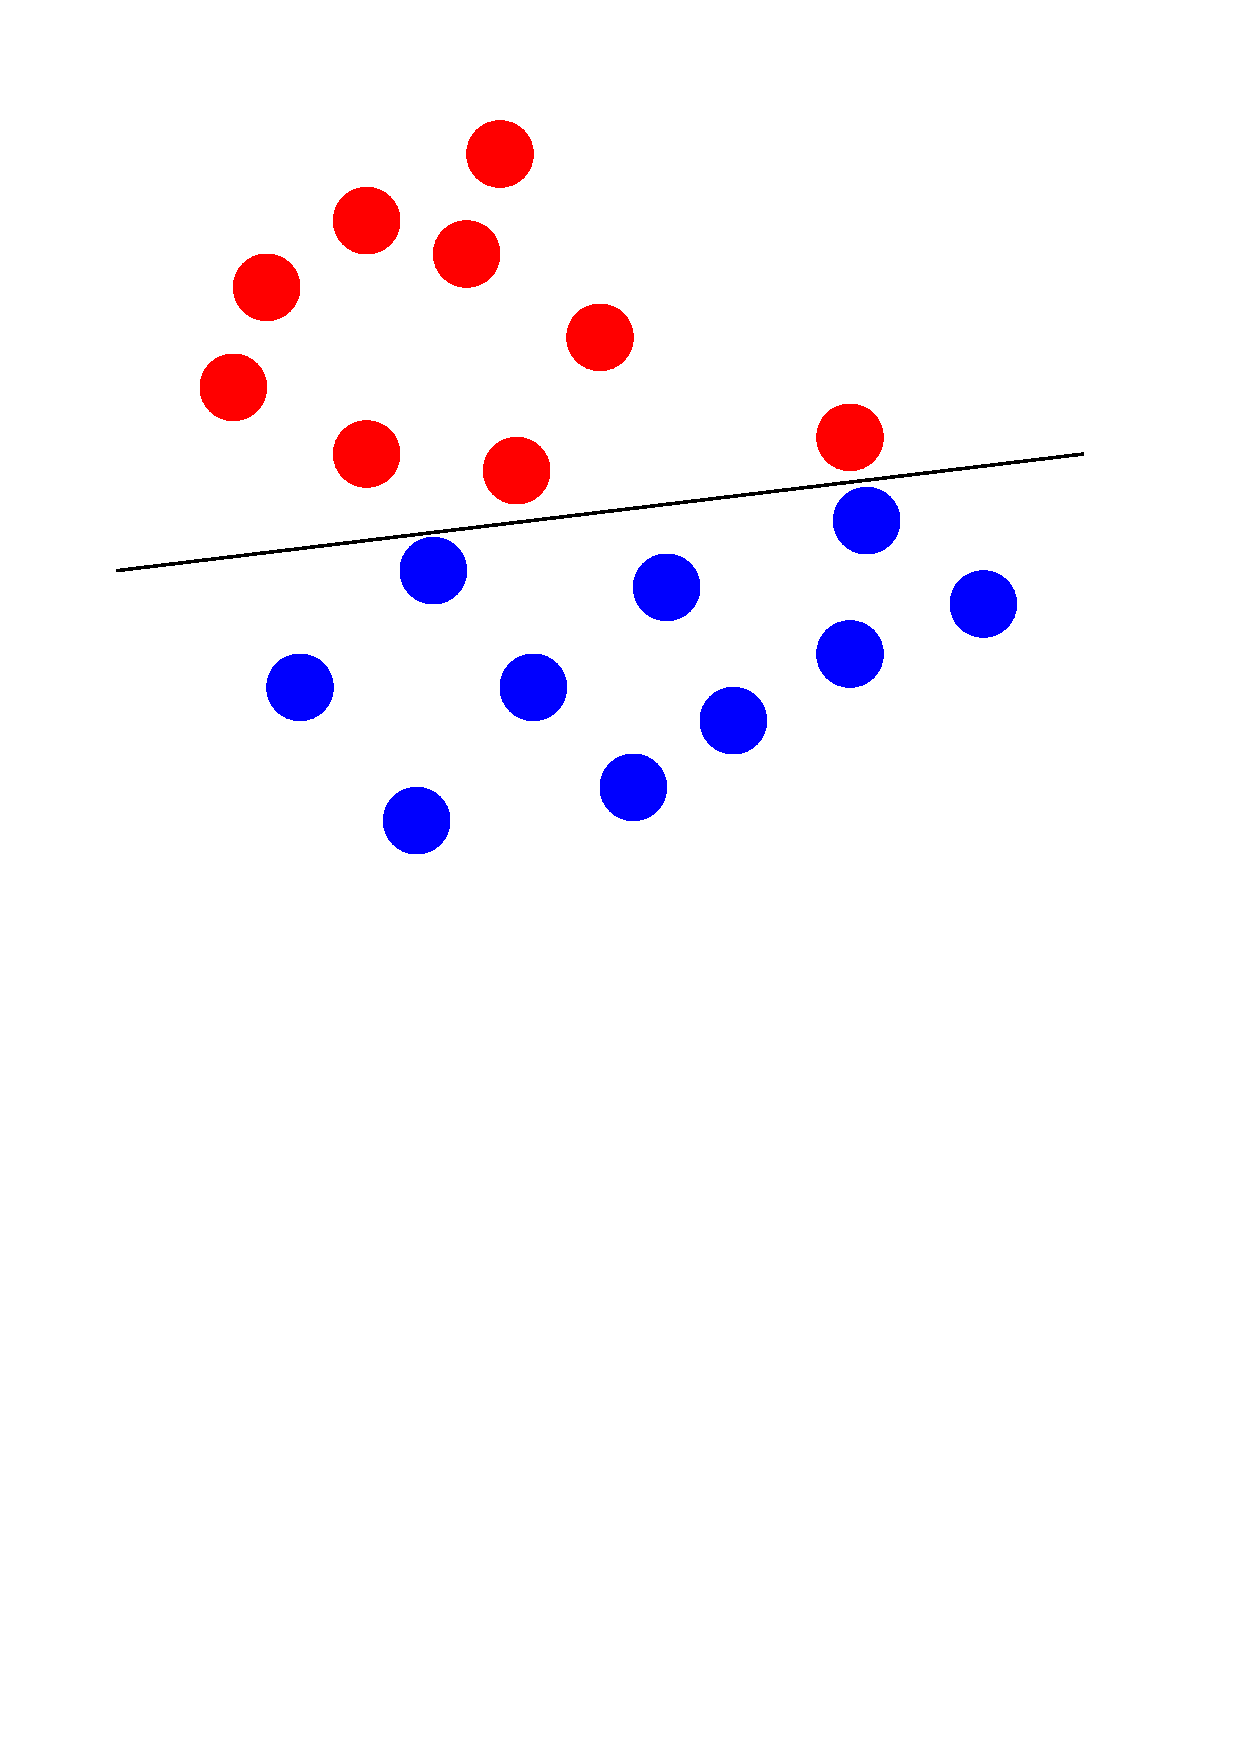
\includegraphics[width=\textwidth]{original}
		\caption{The original data}
		\label{fig:original}
	\end{subfigure}
	\begin{subfigure}{.4\textwidth}
		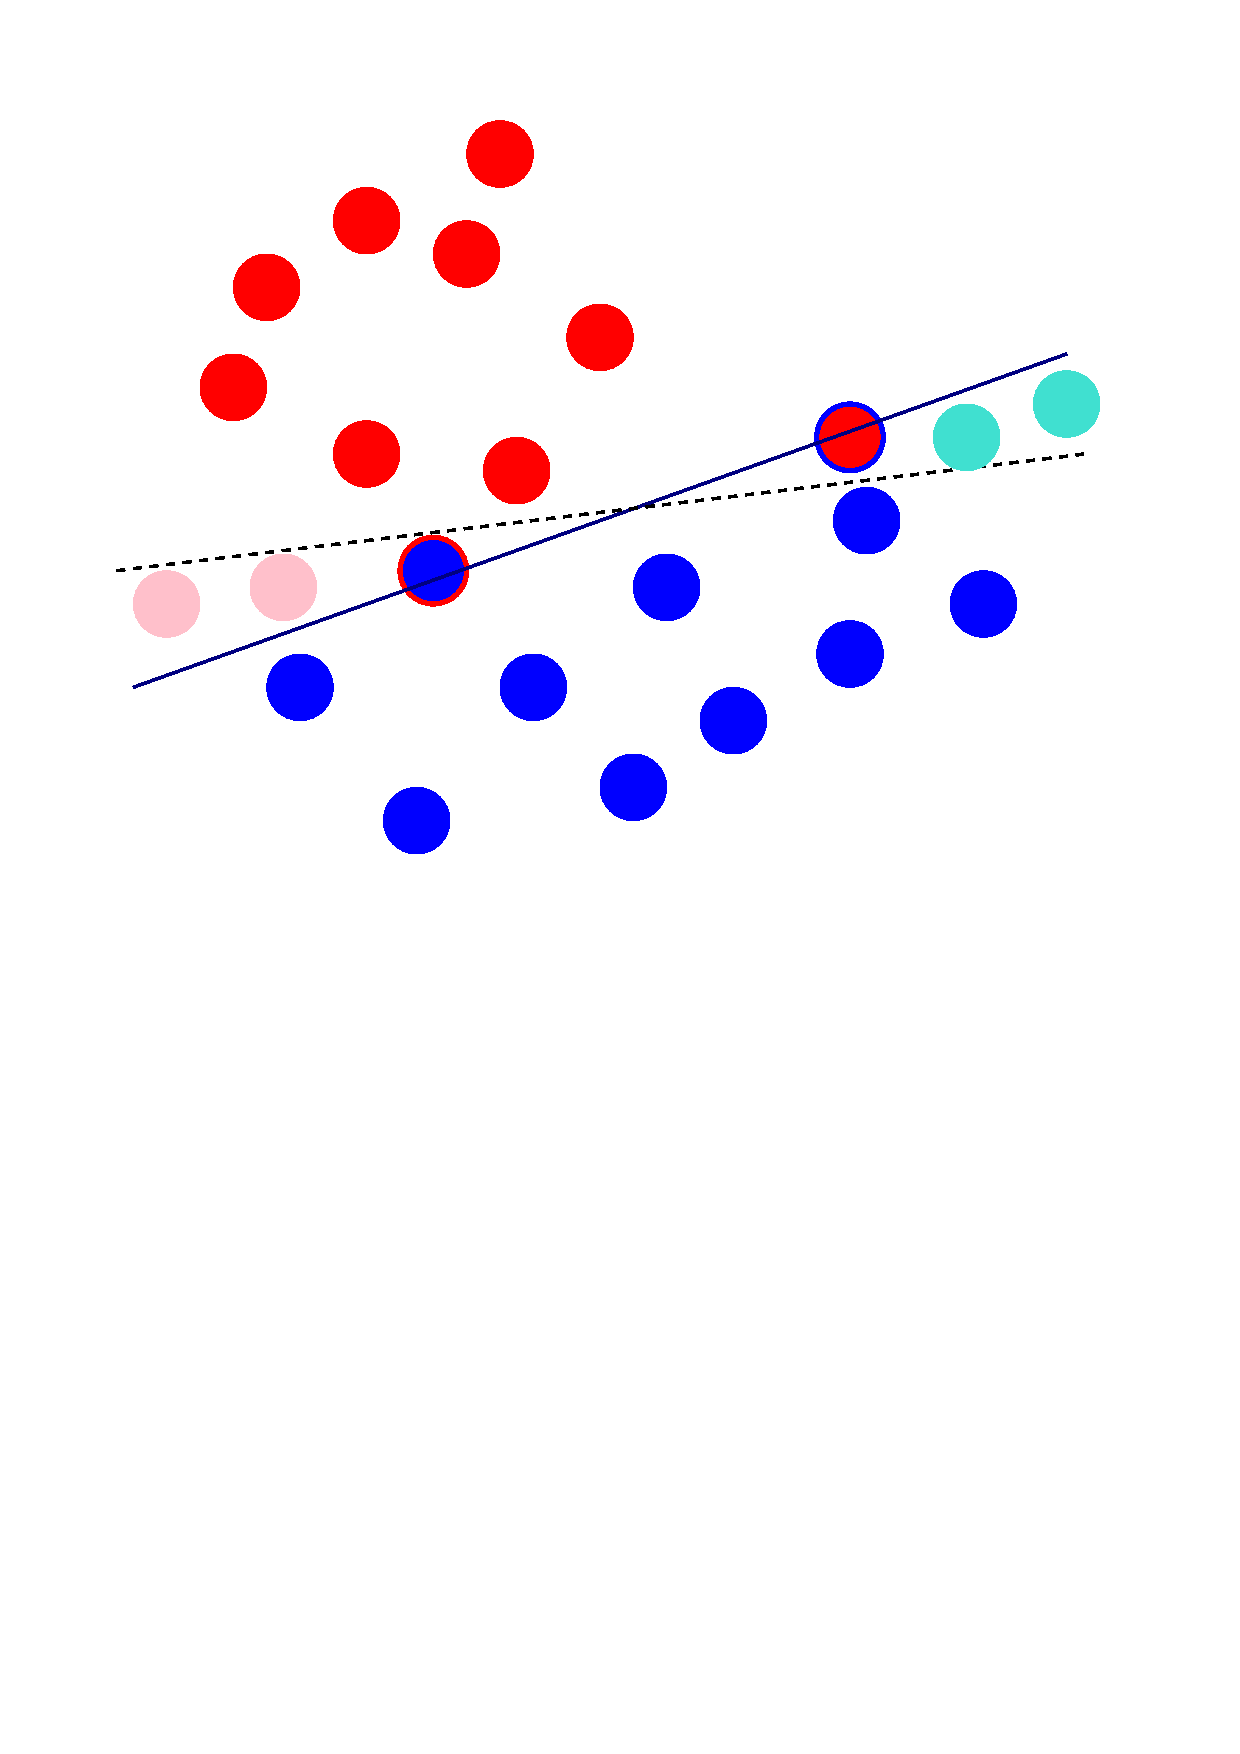
\includegraphics[width=\textwidth]{data_poisoning}
		\caption{Our model}
		\label{fig:poison}
	\end{subfigure}
	\caption{With data poisoning}
	\label{fig:poisoning}
\end{figure}

We can see a representation of this concept in Figure \ref{fig:poisoning}. On the left we have the unattacked system, on the right additional pink points and turquoise points (these are spurious data for the red and blue class respectively) have been used to train the network. This has led to the classification boundaries to change from the dashed line to the solid line, and as a result a blue point and a red point would be misclassified.


\subsection{Literature review}
Maybe this can be done within the previous two sections already?

\section{Description of approaches}

\subsection{Preprocessing techniques}
%In this section, we consider the attack information as noise in the image. We assume attackers tend to control the magnitude of their attacks so as not to be detected by the system, but make them effective enough to misguide the system to the wrong results. We then make use of this effect, and consider the problem from the image preprocessing perspective. We use different approaches, rescaling, bit-depth reduction, total variation and , to remove the attack or adversarial perturbations in the input data before we fit into the net, and also try to maintain enough information for our net to give the right results.

In this section we consider a grey-box setting where the attacker knows the structure of the neural network for the image classifier, however during testing, we impose further transforms on test samples. This is designed to obscure the gradients so that adversarial perturbation effects can be reduced. We looked at a range of preprocessing techniques based on \cite{Guo18}: image resolution reduction, bit-depth reduction, total variation and randomised crop-and-rescale.


\subsubsection{Bit-Depth Reduction} %reference needed here
Bit-Depth reduction approach is to reduce the color depth in bits. We know that each RGB channel has 8-bits, which is possible to be reduced. We then consider removing the noise by reducing the original 8-bit images to fewer bits, as a try to remove the adversarial attack but not significantly destroying the recognisability of the images. 

Before we introduce the way doing bit-depth reduction, we notice that our input values are in the range [0,1]. Then more specifically, for reducing from 8 bits to i bits, we first multiply the input data by ($2^i - 1$),then round to zeros, and scale the values back to the the range [0,1]. Hence we successfully reduce the information capacity from the original 8-bit to i-bit with the critical step of integer rounding. 

\begin{figure}[h!]
	\centering
	\begin{subfigure}{.35\textwidth}
		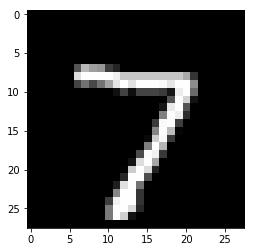
\includegraphics[width=\textwidth]{original7.png}
		\caption{the original image}
		\label{fig: bit-depth reduction 1}
	\end{subfigure}
	\begin{subfigure}{.35\textwidth}
		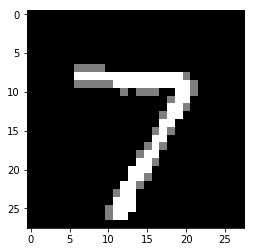
\includegraphics[width=\textwidth]{bit1-7.png}
		\caption{bit-one image}
		\label{fig: bit-depth reduction 8}
	\end{subfigure}
	\caption{Bit-depth reduction image}
\end{figure}

We can see for MNIST database, even we reduce the color depth to just 1 bit, it is very clear and does not introduce human-observable loss. But for images in colored ImageNet, it do shows significant loss when we reduce the bit-depth to be less than 4, which can also be inferred from the decrease in the accuracy in the following results section. 

\subsubsection{Total Variation}


\subsubsection{Image Resolution Reduction}
Most of the time, humans can make out numbers and objects from very low resolution images, this suggests that the defining features of classes are fairly general going from image to image. Therefore intuitively, we expect that if we decrease the resolution by scaling the image to a smaller size then rescaling back, using for example a bilinear interpolation, then the transformed image should still be recognisable (given that the scaling is not too extreme). Since this means there is a local pooling of information, it will be interesting to see if adding such a transformation to all test samples will be more robust against perturbation based attacks.

\subsubsection{Randomised crop and rescaling}
One way of obscuring the gradient of the neural network is to add some random operations during the testing. Randomised crop and rescaling involves taking a random crop of the original image and then rescale back to the desired size. Note that typically a range or proportion is specified so that the image post-cropping can still be recognisable as the original object. 

The neural network is trained on the original images, but when it comes to testing, all test samples are subjected to random transform as described above. Often we take multiple random crop-and-rescaling of the same test image and feed all such transformed images into the neural network. We can then find some summary statistic from all the transformation to classify this image. For example, we can take the mode of the classification or find the maximum of the average sigmoid output value in the final layer of the neural network. 

Of course this means that there are additional computation cost added to the testing phase. However since this is obscured to the attacker, an FGSM attack should be less effective. We also expect that increasing the number of transformed images on a test image should also increase accuracy.



\subsection{Universal adversarial training}

\subsubsection{A brief review of \cite{shafahi_universal_2018}}

Standard white-box adversarial attacks change the predicted class label of an image by tailoring small perturbations to it. On the other hand a universal perturbation attack is an update that can be added to any image (in a broad class) whilst still changing the predicted class label. As of this report there appears to have been little work done in the direction of defending against universal perturbation attacks. A study of this problem hs been carried out by Akhtar et al. \cite{akhtar_defense_2018} in which image pre-processing is usggested as a form of defence but it has been shown that this defense can be easily overcome if the attacker is aware that a defense network is being used \cite{carlini_adversarial_2017}. There is also recent work \cite{perolat_playing_2018} which models the defense as a two-player min-max game. Similar to usual adversarial training they iteratively generate a universal perturbation after each update of the DNN parameters which is very expensive. The approach in \cite{shafahi_universal_2018} also models the defense as a two-player min-max game but with a simple optimisation based universal attack which is much faster and more scalable.

The best known approach for producing universal perturbations is that of Moosavi-Dezfooli et al. \cite{moosavi-dezfooli_universal_2017}, in this one seeks small perturbations which fool the classifier on almost all data points on some sample. For this they search for a pertubation constrained by size (in some $\ell_p$-norm) and that by achieving a quantified fooling rate.  More precisely, given a training set of samples $X=\{ x_i | i=1,...,N \}$ and a network $f(w,\cdot)$ with frozen parameter $w$ it is proposed to find universal perturbations $\delta$ satisfying 
$$\| \delta \| \leq \varepsilon, \quad \text{and} \quad \mathbb{P}(f(w, x) \neq f(w, x + \delta)) \geq 1-\xi,$$
for some given parameter $\xi$. This is then solved by an iterative method, see Algorithm \ref{Alg_1} below, which relies on an expensive inner loop and an outer loop that is not guaranteed to converge.  

%\includegraphics[scale=0.2,angle=-90,origin=c]{Alg_1.pdf}

\begin{algorithm}
\caption{Standard Iterative Solver for Universal Perturbations}\label{Alg_1}
\begin{algorithmic}[1]
%\Procedure{MyProcedure}{}
%\State $\textit{stringlen} \gets \text{length of }\textit{string}$
%\State $i \gets \textit{patlen}$
\State Initialise $\delta \gets 0$

\While{$\mathbb{P}((f(w, x) \neq f(w, x + \delta)) \geq 1-\xi$}  
%\EndWhile

\For{$x_i \in X$} 
%\EndFor

\If{$f(w,x_i+\delta) \neq f(w,x_i)$} \\ 
\hspace{\algorithmicindent} Solve $\min_r \|r\|_2$ s.t.  $f(w,x_i+\delta+r) \neq f(w,x_i)$ by DeepFool \\
\hspace{\algorithmicindent} Update $\delta \gets \delta + r$, then project $\delta$ to $\ell_p$ ball
\EndIf
\EndFor
\EndWhile

%\If{$f(w,x_i+\delta) \neq f(w,x_i)$
%\EndIf

%\If {$i > \textit{stringlen}$} \Return false
%\EndIf
%\State $j \gets \textit{patlen}$

%\If {$\textit{string}(i) = \textit{path}(j)$}
%\State $j \gets j-1$.
%\State $i \gets i-1$.
%\State \textbf{goto} \emph{loop}.
%\State \textbf{close};
%\EndIf
%\State $i \gets i+\max(\textit{delta}_1(\textit{string}(i)),\textit{delta}_2(j))$.
%\State \textbf{goto} \emph{top}.
%\EndProcedure
\end{algorithmic}
\end{algorithm}

In \cite{shafahi_universal_2018} the following optimisation problem is instead considered, 
$$\max_{\delta} \mathcal{L} (w,\delta) = \frac{1}{N} \sum_{i=1}^N \ell(w,x_i + \delta) \quad \text{s.t.} \quad \| \delta \|_p \leq \varepsilon,$$ 
where $\ell$ is a loss function representing the loss used to train a DNN. This simple formulation searches for a universal perturbation which maximises the training loss. Unfortunately in this set-up the cross-entropy loss is unbounded from above which can mean a perturbation that misclassifies just a single image can maximise the above problem. To avoid this it is suggested that one should clip the entropy loss as follows, 
$$\tilde{\ell}(w,x_i + \delta) = \min \{ \ell(w,x_i+\delta), \beta \}.$$ 
This idea is based on a standard stochastic gradient method that comes with convergence guarantees when a decreasing learning rate is used. They directly solve the maximisation problem by SGM, each iteration begins by using gradient ascent to update the universal perturbation to maximise loss, then this perturbation is projected onto the $\ell_p$-norm ball to prevent it from growing too large, this is summarised in Algorithm \ref{Alg_2} below. This method is tested by attacking a naturally trained WideResnet CIFAR-10 model whichh has a clean test accuracy of 95.2\%. They found that accuracies after adding universal perturbation (with $\varepsilon =8$) were 42.56\% for SGD perturbation, 13.08\% for MSGD, 13.3\% for ADAM and 13.17\% for PGD.
\begin{algorithm}
\caption{Standard Iterative Solver for Universal Perturbations}\label{Alg_2}
\begin{algorithmic}[1]
%\State Initialise $\delta \gets 0$

%\While{$\mathbb{P}((f(w, x) \neq f(w, x + \delta)) \geq 1-\xi$}  
%\EndWhile

\For{epoch$-1,...,N_{ep}$} 

\For{minibatch $B \subset X$} \\
\hspace{\algorithmicindent} Update $\delta$ with gradient variant $\delta \gets \delta + g$ \\
\hspace{\algorithmicindent} Project $\delta$ to $\ell_p$ ball


\EndFor
\EndFor
\end{algorithmic}
\end{algorithm}

The next step is to train against universal perturbations, this is done by modelling the problem as a two-player zero sum game. This is formulated as a min-max optimisation problem, $$ \min_w \max_{\delta} \frac1N \sum_{i = 1}^N \ell(w, x_i + \delta) \quad \text{subject to} \quad \| \delta \|_p \leq \varepsilon \, ,$$ where $w$ represents the network weights, $X=\{x_i|i =1,...,N \}$ represents the training samples (of batch size $N$) and $\ell$ is the loss function. The authors propose to solve this problem by alternating stochastic gradient methods, iterating alternate updates of the network weights using gradient descent with updates of the universal perturbation using gradient ascent. Notice here that $w$ and $\delta$ are updated only once per setp with the updates accumulating for both $w$ and $\delta$, in particular there is no expensive inner loop. They found that the following FGSM update rule (for updating $\delta$) was most effective when combined with the SGD optimiser for updating $w$,
$$\text{FGSM} \quad \delta \leftarrow \delta + \varepsilon \, \text{sign}(\mathbb{E}_{x \in B}[\nabla_{\delta} \ell(w, x + \delta)]).$$ 
The training curves for the universal adversarial training process on the Wide Resnet model using the CIFAR-10 dataset is presented. Below we include the first curve of figure 4 of \cite{shafahi_universal_2018} which shows the training cuvre with FGSM used for the universal perturbation maximisation.
\begin{figure}[b] 
\caption{The training cuvre with FGSM used for the universal perturbation maximisation}
%\includegraphics[scale=.41,angle=-90,origin=c]{Fig_4.pdf}
\centering
\end{figure}
\begin{algorithm}
\caption{Adversarial Training for Universal Perturbations}\label{Alg_3}

 \textbf{Input}: : Training samples $X$, perturbation bound $\varepsilon$, learning rate $\tau$, momentum $\mu$ \\
\begin{algorithmic}[1]
%\State Initialise $\delta \gets 0$


%\While{$\mathbb{P}((f(w, x) \neq f(w, x + \delta)) \geq 1-\xi$}  
%\EndWhile

\For{epoch$-1,...,N_{ep}$} 

\For{minibatch $B \subset X$} \\
\hspace{\algorithmicindent} Update $w$ with momentum stochastic gradient \\
\hspace{\algorithmicindent} \hspace{\algorithmicindent} $g_w \gets \mu g_w - \mathbb{E}_{x \in B} [\nabla_w \ell(w,x+\delta)]$ \\
\hspace{\algorithmicindent} \hspace{\algorithmicindent} $w \gets w + \tau g_w$ \\
\hspace{\algorithmicindent} Update $\delta$ with stochastic gradient ascent \\
\hspace{\algorithmicindent} \hspace{\algorithmicindent} $\delta \gets \delta + \varepsilon \text{sign}(\mathbb{E}_{x \in B}[\nabla_{\delta} \ell(w,x + \delta)])$ \\
\hspace{\algorithmicindent} Project $\delta$ to $\ell_p$ ball


\EndFor
\EndFor
\end{algorithmic}
\end{algorithm}

To test the robustness the authors compare the universally trained model's robustness with other hardened models against white-box attacks. These models are attacked with both universal perturbation attacks and per-instance attacks, specifically FGSM, R-FGSM and PGD (projected gradient descent) are used. It is important to remark that PGD is an attack which iteratively applies FGSM multiple times and is considered to be one of the strongest per-instance attacks. There are models which are PGD trained and effective, but this is time consuming and does not appear to scale well. The White-box performance of hardened WideResnet models trained on CIFAR-10 are shown in figure \ref{table} below.
%\begin{wrapfigure}{r}{0.25\textwidth}
   % \centering
    %\includegraphics[width=0.25\textwidth,scale=.3]{blackboxtable_1.png}
%\end{wrapfigure} 
As one can see the model is most robust against universal perturbation attacks as one would expect. Interestingly it has moderate robustness against PGD attacks whilst having similar computational costs to the non-iterative FGSM and R-FGSM attacks both of which PGD fools almost every time. 
\begin{figure}[b] \label{table}
\caption{ The White-box performance of hardened WideResnet models trained on CIFAR-10}
%\includegraphics[width=7.5cm]{blackboxtable_1.png}
\centering
\end{figure}

%\includegraphics[scale=.41,angle=-90,origin=c]{blackboxtable_1.pdf}

Robustness of the universally trained model in the black-box attack scenario is also tested. It is found that they are also quite resistant to black-box per-instance attacks – achieving resistance comparable to 7-step PGD adversarial training at a fraction of the cost. Furthermore, per-instance adversarial examples built to attack the universally hardened model transfer to other black-box models very well.

\subsection{Detection}

%{\bf Input from John.}

We examine the problem of detecting adversarial attacks, focusing on the simple class of FGSM adversarial attacks as defined in \eqref{eq:fgsm}.

\subsubsection{Problem Set-up}\label{Setup}

FGSM attacks are constructed by perturbing a non-adversarial image with a fixed level of noise $\varepsilon \in \mathbb{R}$ up to the sign of the loss function $L$ with respect to the feature space $x$:
\begin{equation}
\mathbf{\tilde{X}}=\mathbf{X} + \text{sign}{\nabla_x L(\theta,\mathbf{X},y)}\cdot\varepsilon,
\end{equation}
where $\mathbf{X} \in \mathbb{R}^n$ is the flattened image and $y$ is the true class label. $\varepsilon$ is chosen to be sufficiently small to make detection of image tampering invisible to the human eye, but sufficiently large to induce an incorrect classification by the neural network. Given the nature of the perturbation, it is clear that this class of attack is available to attackers only if they have access to the analytic form of the loss function associated with the neural network they are attacking. 

\par 

We consider identifying FGSM attacks for a network a four-layer network consisting of two convolutional layers followed by two fully-connected layers. The first convolutional layer takes as input a one-channel, $28\times 28$ image and outputs five channels based on a $5\times 5$ kernel. The second layer outputs 20 channels, also based on a $5\times 5$ kernel, with randomly-selected dropouts. We apply max-pooling to $2\times 2$ grids of the output of each convolutional layer. The first fully-connected layer takes as input a vector $\in \mathbb{R}^{320}$ and outputs in $\mathbb{R}^{50}$, before applying a ReLu activation function to this output. The final layer uses a log-softmax function to output the classification probabilities. We consider the MNIST dataset; thus the output of the final layer is $\in [0,1]^{10}$.

\subsubsection{Approach}

We trained the neural network described in Section \ref{Setup} on MNIST training data, containing 60,000 examples of handwritten digits in 0-9.  Using the FGSM approach with $\varepsilon =\{0.05,0.1,0.15,0.2,0.25,0.3\}$ we find about 45,000 successful adversarial examples for our network and data set.
\par
We next choose a subset of 8,000 images from the training set and pass these through the net, obtaining the vectorised features $\boldsymbol{\phi}_{j}$ from each layer $j=\overline{1,4}$. We then train a linear PCA dimensionality reduction model $M_j$ for each layer using these $\boldsymbol{\phi}_j$. For each layer, we keep the first $n_j$ principal components such that we retain approximately 90\% of the variance in the data. This gives $(n_1, n_2, n_3, n_4) = (75, 55, 12, 12)$. We show in Figure \ref{fig:PCA} the fractional variance and cumulative variance captured by each principal component for each layer.

\begin{figure}
\centering
\begin{subfigure}{.5\textwidth}
  \centering
  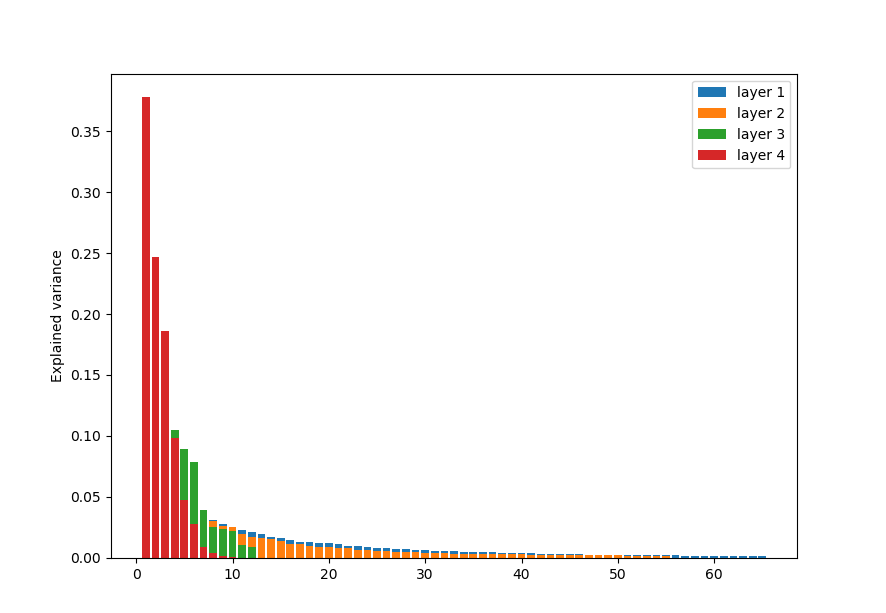
\includegraphics[width=.6\linewidth]{ExplainedVarianceLegend.png}
  \caption{Explained variance of principal components}
  \label{fig:PCA1}
\end{subfigure}%
\begin{subfigure}{.5\textwidth}
  \centering
  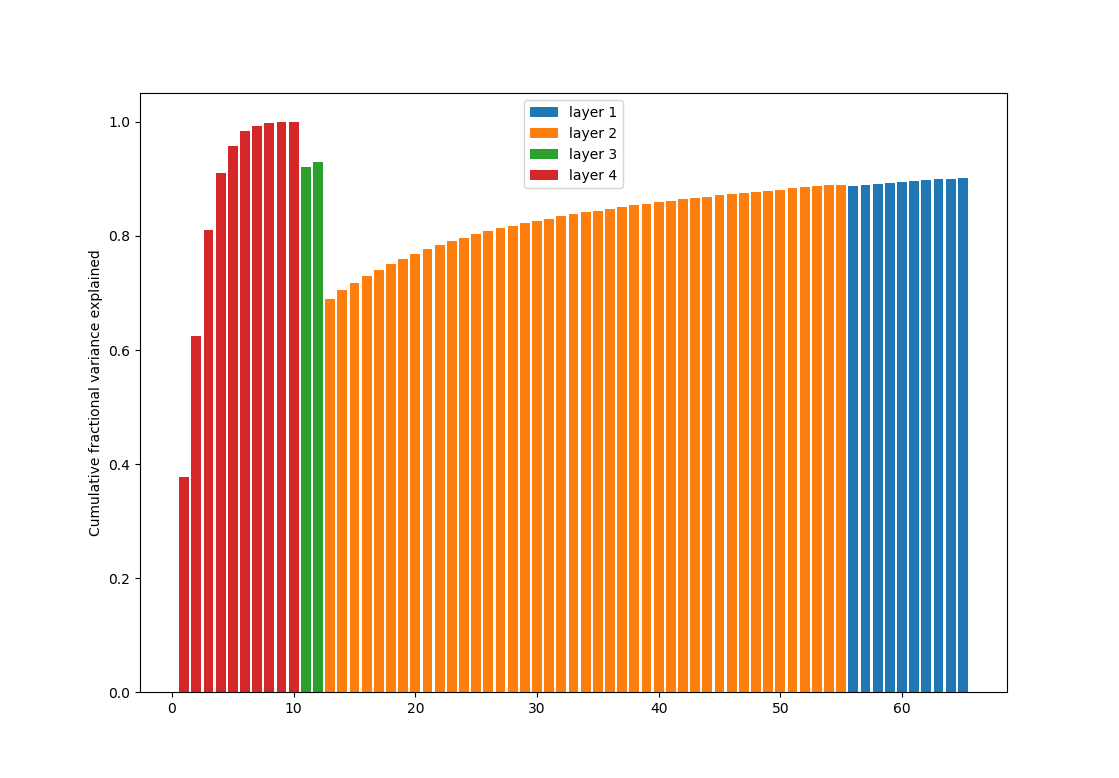
\includegraphics[width=.4\linewidth]{CumExplainedVarianceLegend.png}
  \caption{Cumulative explained variance of principal components}
  \label{fig:PCA2}
\end{subfigure}
\caption{}
\label{fig:PCA}
\end{figure}
Note that this does not require access to the adversarial attacks. For each layer we next train a k-nearest neighbour model on the uncorrupted data, with $k=20$, and using the reduced dimension space found with PCA. For all the test examples we will thus find the closest 20 neighbours from the training data, and the corresponding distances.  We use this to compute the Local intrinsic dimensionality (LID) (REFERENCE NEEDED) for each data point, in each layer. Thus, each data sample is now characterised by $\mathbf{l}_i \in \mathbb{R}^4$, corresponding to the four layers. We consider the practical approximation of LID, defined as (REFERENCE)
\begin{equation}
LID(x) = -\left(\frac{1}{k}\sum_{i=1}^{k}\log\frac{r_i(x)}{r_k(x)}\right)^{-1},
\end{equation}
where $r_i(x)$ denotes the distance between $x$ and its $i$ nearest neighbour within the 8,000 uncorrupted data points, and $r_k(x)$ is the maximum of these values. Note that in our case $x$ corresponds to the reduced feature vector of each datapoint, for each layer.

We next randomly choose a subset of about 8,000 successful adversarial examples, together with the training set. We train a classifier $\mathcal{C}$ that takes as input for each data point the LID vector $\mathbf{l}_i$ and outputs $y=1$ if the example is adversarial and $0$ otherwise. We consider Logistic Regression and SVM for $\mathcal{C}$.

\section{Description of results}

\subsection{Preprocessing techniques}
In this section, we have implemented the preprocessing techniques we described above to different level of attacks, to be more specific the $\epsilon$ in FGSM attack. We then plot the accuracy of our net, with various values of parameters in different techniques.

\subsubsection{Bit-Depth Reduction}

\begin{figure}[h!]
	\centering
	\begin{subfigure}{.4\textwidth}
		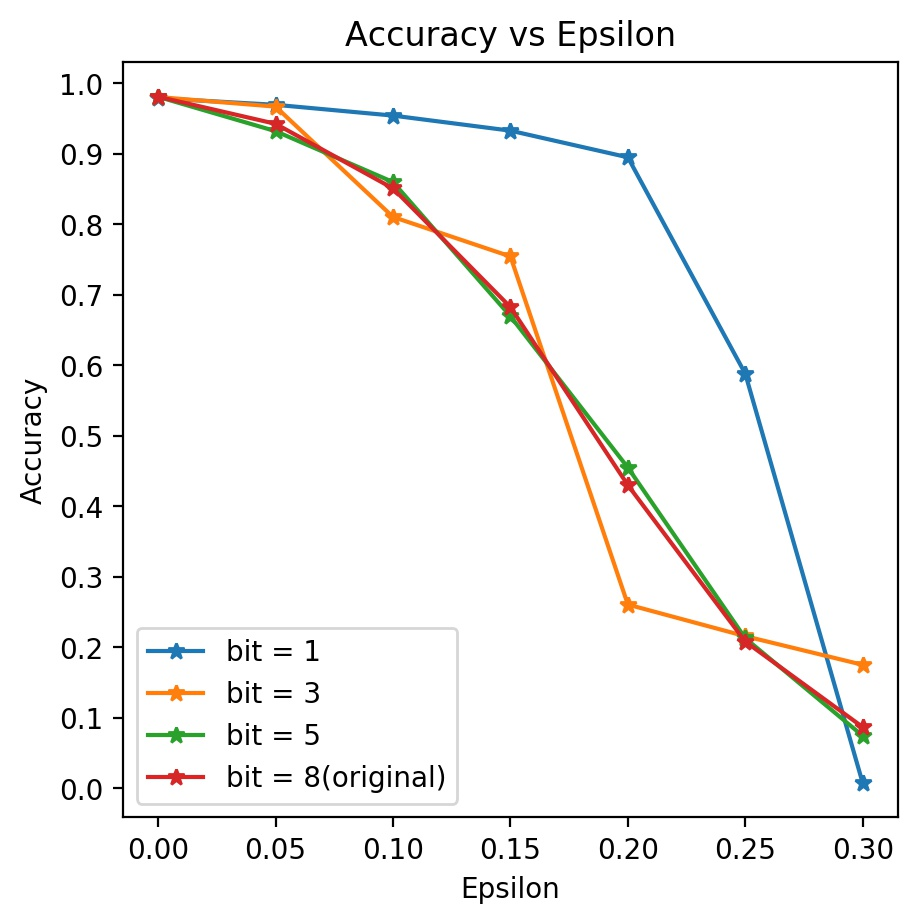
\includegraphics[width=\textwidth]{pretrained_Accuracy_vs_Epsilon_db.jpg}
		\caption{pretrained model}
		\label{fig: bit-depth reduction pre}
	\end{subfigure}
	\begin{subfigure}{.4\textwidth}
		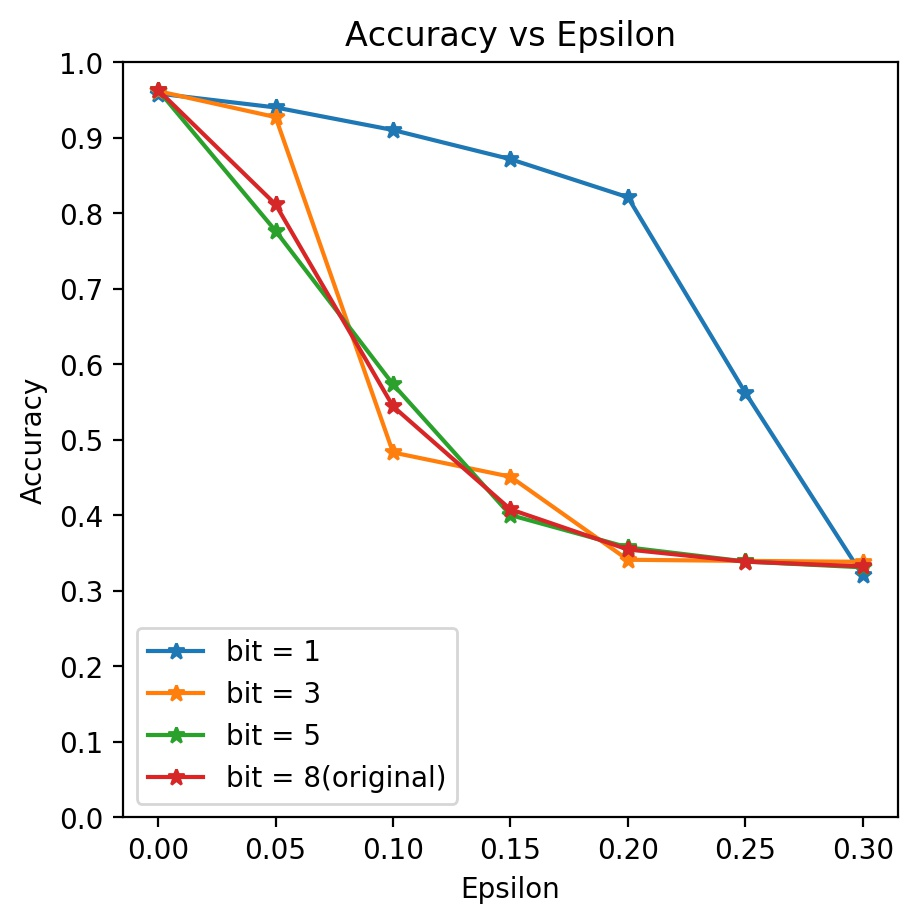
\includegraphics[width=\textwidth]{Accuracy_vs_Epsilon_db.jpg}
		\caption{Our model}
		\label{fig: bit-depth reduction us}
	\end{subfigure}
	\caption{Accuracy for different levels of noise we choose}
\end{figure}



\subsubsection{Total Variation}
\begin{figure}[h!]
	\centering
	\begin{subfigure}{.4\textwidth}
		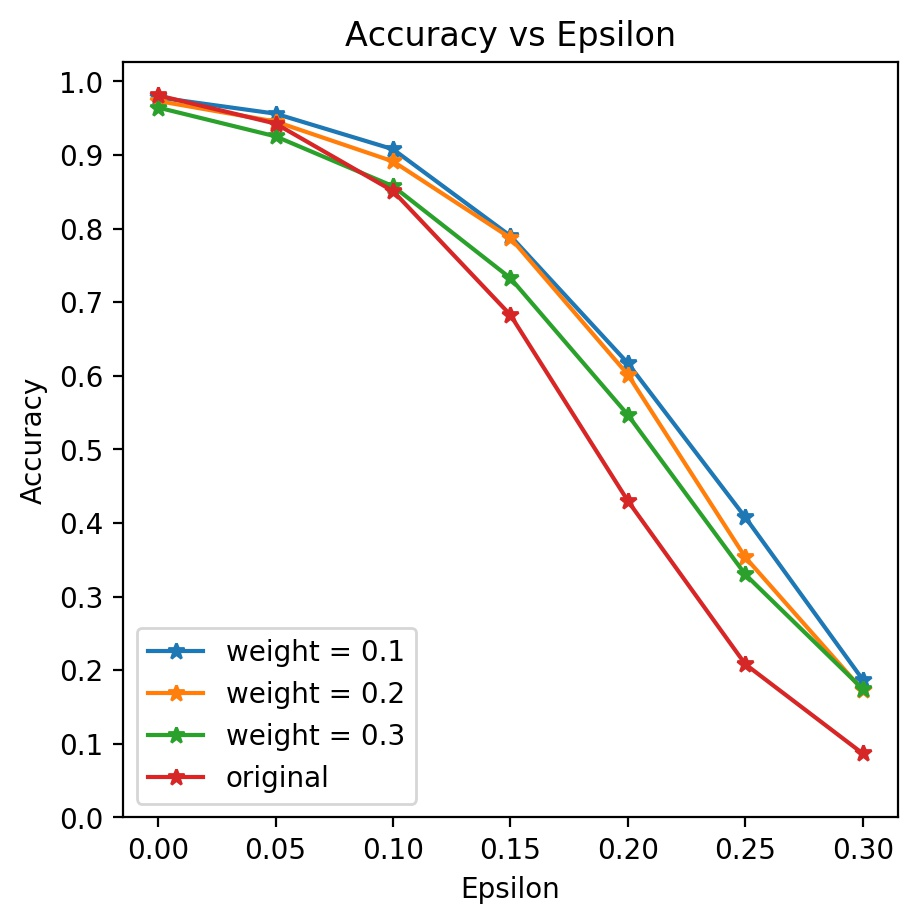
\includegraphics[width=\textwidth]{pretrained_Accuracy_vs_Epsilon_tv.jpg}
		\caption{pretrained model}
		\label{fig: tv pre}
	\end{subfigure}
	\begin{subfigure}{.4\textwidth}
		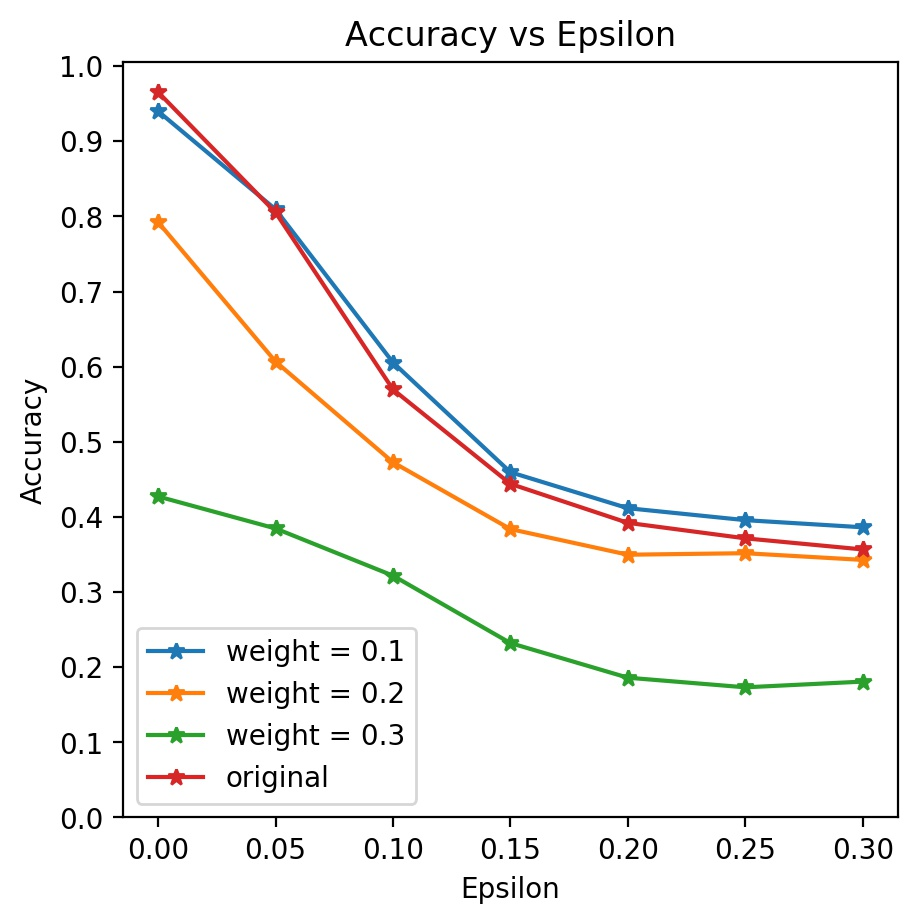
\includegraphics[width=\textwidth]{Accuracy_vs_Epsilon_tv.jpg}
		\caption{Our model}
		\label{fig: tv us}
	\end{subfigure}
	\caption{Accuracy for different levels of noise we choose}
\end{figure}

\subsection{Universal adversarial training}

\subsection{Detection}

By training the two classifiers (SVM and Logistic Regression) we obtain very similar results. In both cases the training accuracy is very close to, or even $100\%$. We do multiple runs since the data used to train $\mathcal{C}$ is drawn at random. This suggests that the decision boundary is very far from the regions of interest for the two classes, meaning that the LID is a good measure for detecting adversarial attacks. We next considering a test set, composed of about 2,000 images for each of the adversarial and non-adversarial attacks. We obtain no false positives on either of the classifiers, and a single false negative. This is shown in Figure .
\begin{figure}
\centering
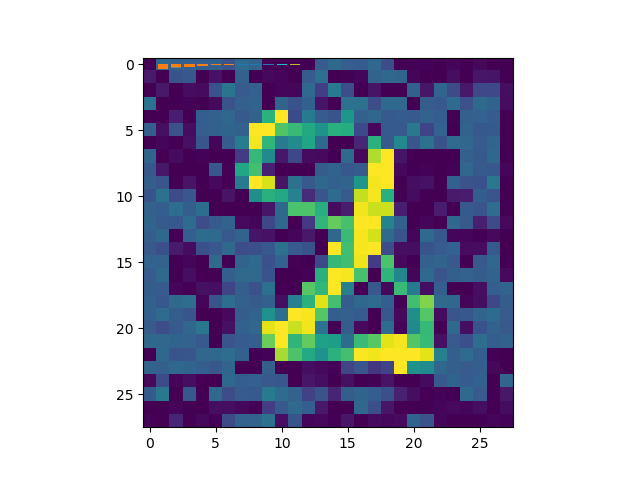
\includegraphics[scale=0.8]{eightthree.png}
\caption{Perturbed image of 8, misclassified as a 3.}
\end{figure}
We note that we have also tried training the classifiers directly on the PCA reduced features for each layer, $\mathbf{x} =(\boldsymbol{\phi}_1,\boldsymbol{\phi}_2,\boldsymbol{\phi}_3,\boldsymbol{\phi}_4)$, but we obtain performance that is only slightly better than random, for both the training and the test stages. This means that this feature vector is not appropriate for capturing whether the data is adversarial or not. This also confirms that LID is an appropriate measure for this.

\section{Conclusions \& outlook}

\subsection{Preprocessing techniques}

\subsubsection{Defence GAN}
The Defence GAN approach appears promising, despite our inability to replicate recent results.  There are however a number of areas that are yet to be fully explored.  An interesting comparative approach would be to replace the GAN based generator with an autoencoder based model.  This has particular benefits in terms of training as GANs are notoriusly difficult to train and for larger more diverse datasets the easier training method might be more desirable if prediction accuracy doesn't decrease with the blurrier images generated by variational autoencoders.

The other important area to invesitgate is the nature of the algorithm used to align the generated image with the semantic visual content of the poisoned image.  At present method is to minimise the pixel-wise distance between the generated image and the poisoned image by performing regression on the randomly sampled input vector for the generator.  At classification time this is the method that does most of the heavy lifting and perhaps improving this may improve results or simply speed up classification.  One potential approach if we use an autoencoder is to use the bottleneck layers output to initialise our input vector, potentially using the predicted values as the means for a gaussian we sample from.

\subsubsubsection{Combining Approaches}
A number of the pre-processing techniques are promising in their own right. Combining the techniques may provide added security.  One such approach could combine pre-processing techniques, such as rescaling with the autoencoder approach, to remove the attack before it is passed to the autoencoder, with the auto-encoder trained to regenerate the un-processed image.  There are a number of possibilities here, some more costly in terms of classification time than others.

\subsection{Universal adversarial training}

Based on the universal adversarial training technique of \cite{shafahi_universal_2018} that we reviewed above and started to implement ourselves we have several suggestions as to how one might continue research in this direction. 

% Firstly one could consider ... . We consider an image classifier $f_c(w_c,\cdot)$ with system variables $w_c$ and loss function $\ell_c(w_c, \cdot, \cdot)$. On the other hand consider an attacker $f_a(w_a,\cdot)$ ... 

% \begin{algorithm}
% \caption{Adversarial Training for Universal Perturbations 2.0}\label{Alg_4}

%  \textbf{Input}: : Training samples $X$, perturbation bound $\varepsilon$, learning rate $\tau$, momentum $\mu$ \\
% \begin{algorithmic}[1]
% %\State Initialise $\delta \gets 0$


% %\While{$\mathbb{P}((f(w, x) \neq f(w, x + \delta)) \geq 1-\xi$}  
% %\EndWhile

% \For{epoch$-1,...,N_{ep}$} 

% \For{minibatch $B \subset X$} \\
% \hspace{\algorithmicindent} Update $w$ with momentum stochastic gradient \\
% \hspace{\algorithmicindent} \hspace{\algorithmicindent} $g_c \gets \mu_c g_c - \mathbb{E}_{x \in B} [\nabla_{w_c} \ell(w_c,f_a(w_a,x+\delta))]$ \\
% \hspace{\algorithmicindent} \hspace{\algorithmicindent} $w_c \gets w_c + \tau_c g_{w_c}$ \\
% \hspace{\algorithmicindent} Update $\delta$ with stochastic gradient ascent \\
% \hspace{\algorithmicindent} \hspace{\algorithmicindent}  $g_a \gets \mu_a g_a - \mathbb{E}_{x \in B} [\nabla_{w_a} \ell(w_a,f_c(w_c,x+\delta))]$ \\
% \hspace{\algorithmicindent} \hspace{\algorithmicindent} $w_a \gets w_a + \tau_a g_{w_a}$
% \EndFor
% \EndFor
% \end{algorithmic}
% \end{algorithm}

For a potential extension of the universal adversarial training model one could replace the perturbation with a GAN, i.e.

$$ \min_{w_1} \max_{w_2} \frac1N \sum_{i = 1}^N \ell(w_1, x_i + D(w_2)) ,$$

where $D$ denotes the generative network. One important aspect that needs to be guaranteed is that the output layer of this network ensures that the output is bounded (for example in terms of an $\ell^p$-ball of radius $\varepsilon$). 

\subsection{Detection}

%-------------------------------------------------------------------------------
% References
%-------------------------------------------------------------------------------

\bibliographystyle{unsrt}
\bibliography{dstl.bib}

\end{document}
